\documentclass[twoside,11pt,a4paper]{article}

\usepackage[utf8]{inputenc}
\usepackage{amsmath, amssymb, latexsym}

\usepackage{tikz}
\usepackage{pgfplots}

\begin{document}
	\begin{figure}
		\centering
		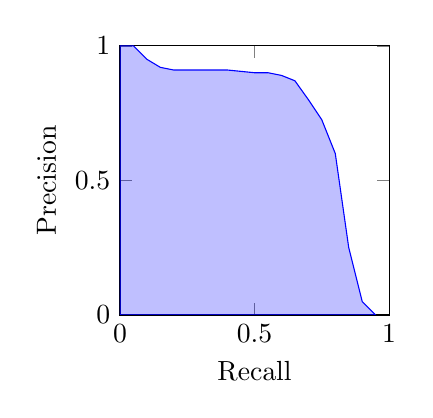
\begin{tikzpicture}
			\begin{axis}[
						height=5cm,
						width=5cm,
						xlabel=Recall,
						ylabel=Precision,
						xtick={0,0.5,1},
						ytick={0,0.5,1},
						ymin=0,
						ymax=1,
						xmin=0,
						xmax=1]
					
				\addplot[fill=blue,fill opacity=0.25,blue,mark=none] coordinates {
					(0,1)
					(0.05,1)
					(0.1,0.95)
					(0.15,0.92)
					(0.2,0.91)
					(0.3,0.91)
					(0.4,0.91)
					(0.5,0.9)
					(0.55,0.9)
					(0.6,0.89)
					(0.65,0.87)
					(0.7,0.8)
					(0.75,0.725)
					(0.8,0.6)
					(0.85,0.25)
					(0.9,0.05)
					(0.95,0)
				} -| (current plot begin);
			\end{axis}
		\end{tikzpicture}
	\end{figure}
\end{document}